\documentclass[a4paper,12pt]{article}
\usepackage[utf8]{inputenc}
\usepackage{amsmath}
\usepackage{listings}
\usepackage{geometry}
\geometry{margin=2.5cm}
\usepackage{graphicx}
\usepackage{xcolor}
\title{Questionnaire complet – IDS AI System}
\author{Projet Tutored}
\date{\today}

\lstdefinelanguage{JavaScript}{
  keywords={break, case, catch, continue, debugger, default, delete, do, else, finally, for, function, if, in, instanceof, new, return, switch, this, throw, try, typeof, var, void, while, with, let, const},
  keywordstyle=\color{blue}\bfseries,
  ndkeywords={class, export, boolean, throw, implements, import, this},
  ndkeywordstyle=\color{darkgray}\bfseries,
  identifierstyle=\color{black},
  sensitive=false,
  comment=[l]{//},
  morecomment=[s]{/*}{*/},
  commentstyle=\color{gray}\ttfamily,
  stringstyle=\color{red}\ttfamily,
  morestring=[b]',
  morestring=[b]", 
  morestring=[b]`
}

\begin{document}

\maketitle

\tableofcontents

\newpage

%%%%%%%%%%%%%%%%%%%%%%%%%%%%%%%%%%%%%%%%%%%%%%%%%%%%%%%%%%%%
\section{Introduction}

Ce document répond à toutes les questions essentielles sur le projet \textbf{IDS AI System}, qui combine une intelligence artificielle (Deep Learning) pour la détection d’intrusions réseau et une interface web moderne (Next.js).  
Chaque question est suivie d’une explication claire, d’exemples de code, et d'illustrations pour permettre à tout étudiant de comprendre le fonctionnement du projet.

%%%%%%%%%%%%%%%%%%%%%%%%%%%%%%%%%%%%%%%%%%%%%%%%%%%%%%%%%%%%
\section{Fondamentaux : Machine Learning et Deep Learning}

\subsection{Qu'est-ce que le Machine Learning ?}
Le Machine Learning (apprentissage automatique) regroupe les techniques où l’ordinateur apprend à partir de données, sans être explicitement programmé pour chaque tâche. Il s'agit par exemple de reconnaître des motifs ou de faire des prédictions à partir d'exemples.

\subsection{Qu'est-ce que le Deep Learning ?}
Le Deep Learning (apprentissage profond) est une branche du Machine Learning qui utilise des réseaux de neurones comportant plusieurs couches cachées. Cela permet au modèle de comprendre des relations très complexes dans les données, comme reconnaître des attaques réseau à partir de nombreux paramètres.

\subsection{Différences entre Machine Learning et Deep Learning}
La principale différence réside dans la profondeur et la capacité du modèle :
\begin{itemize}
  \item Le Machine Learning classique utilise souvent des modèles plus simples (arbres de décision, SVM, régressions, etc.) et nécessite beaucoup de travail manuel pour choisir les bonnes variables (features).
  \item Le Deep Learning automatise l'extraction des caractéristiques grâce à ses couches successives, et peut traiter des données brutes ou très complexes.
\end{itemize}
Dans ce projet, on utilise un modèle Deep Learning de type CNN-LSTM, capable d'apprendre automatiquement des motifs dans le trafic réseau.

%%%%%%%%%%%%%%%%%%%%%%%%%%%%%%%%%%%%%%%%%%%%%%%%%%%%%%%%%%%%
\section{Architecture du modèle IA}

\subsection{Présentation générale}
Le modèle utilisé dans ce projet est un réseau de neurones profond qui combine deux types d'architectures :
\begin{itemize}
  \item \textbf{CNN (Convolutional Neural Network)} : pour repérer des motifs locaux dans les séquences de données réseau.
  \item \textbf{LSTM (Long Short-Term Memory)} : pour mémoriser des séquences et détecter des comportements anormaux sur la durée.
\end{itemize}
Les données passent d'abord par des couches de convolution 1D, puis par des couches LSTM, et enfin par des couches entièrement connectées (denses) avant d'arriver à la sortie.

\subsection{Nombre de couches et de neurones}
Le modèle comporte :
\begin{itemize}
  \item 2 couches de convolution (64 et 128 filtres)
  \item 2 couches LSTM (128 et 64 neurones)
  \item 2 couches denses (128 et 64 neurones)
  \item 1 couche de sortie (nombre de neurones = nombre de classes, ici 9)
\end{itemize}

\textbf{Calcul du nombre total de neurones (hors batchnorm, dropout, etc.) :}
\begin{itemize}
  \item Conv1D-1 : 64 filtres
  \item Conv1D-2 : 128 filtres
  \item LSTM-1 : 128 neurones
  \item LSTM-2 : 64 neurones
  \item Dense-1 : 128 neurones
  \item Dense-2 : 64 neurones
  \item Sortie : 9 neurones
\end{itemize}
\textbf{Total (hors redondance) :} 64 + 128 + 128 + 64 + 128 + 64 + 9 = \textbf{585 neurones}

\subsection{Caractéristiques du réseau de neurones}
\begin{itemize}
  \item \textbf{Fonctions d'activation :} ReLU pour les couches cachées, Softmax pour la sortie.
  \item \textbf{Normalisation :} BatchNormalization après chaque convolution et dense.
  \item \textbf{Régularisation :} Dropout (0.25 ou 0.5) pour éviter le surapprentissage.
  \item \textbf{Architecture séquentielle :} Les couches sont empilées les unes après les autres.
\end{itemize}

\subsection{Extrait de code du modèle}
\begin{lstlisting}[language=Python]
model = models.Sequential([
    layers.Input(shape=self.input_shape),
    layers.Conv1D(64, 3, activation='relu', padding='same'),
    layers.BatchNormalization(),
    layers.Conv1D(128, 3, activation='relu', padding='same'),
    layers.BatchNormalization(),
    layers.MaxPooling1D(2),
    layers.Dropout(0.25),
    layers.LSTM(128, return_sequences=True),
    layers.Dropout(0.25),
    layers.LSTM(64),
    layers.Dropout(0.25),
    layers.Dense(128, activation='relu'),
    layers.BatchNormalization(),
    layers.Dropout(0.5),
    layers.Dense(64, activation='relu'),
    layers.BatchNormalization(),
    layers.Dropout(0.5),
    layers.Dense(self.num_classes, activation='softmax')
])
\end{lstlisting}

\subsection{Résumé sous forme de tableau}
\begin{tabular}{|c|c|c|}
\hline
Type de couche & Nombre de neurones/filtres & Activation \\
\hline
Conv1D & 64 & ReLU \\
Conv1D & 128 & ReLU \\
LSTM & 128 & - \\
LSTM & 64 & - \\
Dense & 128 & ReLU \\
Dense & 64 & ReLU \\
Dense (sortie) & 9 & Softmax \\
\hline
\end{tabular}

%%%%%%%%%%%%%%%%%%%%%%%%%%%%%%%%%%%%%%%%%%%%%%%%%%%%%%%%%%%%
\section{Données utilisées}

\subsection{Données d'entrée}
Les données d'entrée sont issues du jeu de données NSL-KDD, un standard pour la détection d’intrusions réseau. Chaque exemple correspond à une connexion réseau décrite par de nombreux paramètres (adresses IP, ports, protocole, etc.).

\subsection{Prétraitement des données}
Avant d'être utilisées par le modèle, les données subissent plusieurs transformations :
\begin{itemize}
  \item Les variables textuelles (catégorielles) sont converties en variables numériques (one-hot encoding).
  \item Les valeurs sont normalisées (StandardScaler) pour que toutes les features soient sur la même échelle.
  \item Les labels (types d'attaque) sont encodés en one-hot.
\end{itemize}

\begin{lstlisting}[language=Python]
categorical_columns = X.select_dtypes(include=['object']).columns
X = pd.get_dummies(X, columns=categorical_columns)
scaler = StandardScaler()
X_scaled = scaler.fit_transform(X)
label_encoder = LabelEncoder()
y_encoded = label_encoder.fit_transform(y)
y_categorical = to_categorical(y_encoded)
\end{lstlisting}

\subsection{Données de sortie}
Le modèle prédit la classe d'attaque parmi 9 catégories :
\begin{lstlisting}[language=Python]
ATTACK_TYPES = {
    0: 'Normal',
    1: 'DoS',
    2: 'Probe',
    3: 'R2L',
    4: 'U2R',
    5: 'SQL Injection',
    6: 'XSS',
    7: 'Port Scan',
    8: 'Brute Force'
}
\end{lstlisting}

\subsection{Provenance des données de test}
Dans ce projet, le fichier utilisé est \texttt{NSL-KDD-Train.csv}. Il n'y a pas de jeu de test séparé fourni dans le dossier, mais une partie des données est réservée à la validation (20\% par défaut).

%%%%%%%%%%%%%%%%%%%%%%%%%%%%%%%%%%%%%%%%%%%%%%%%%%%%%%%%%%%%
\section{Entraînement et hyperparamètres}

\subsection{Hyperparamètres utilisés}
\begin{itemize}
  \item Optimiseur : Adam
  \item Fonction de perte : categorical	extunderscore crossentropy
  \item Epochs : 50
  \item Batch size : 32
  \item EarlyStopping (patience=5)
  \item ReduceLROnPlateau (patience=3, factor=0.2)
\end{itemize}

\begin{lstlisting}[language=Python]
history = self.model.fit(
    X_train, y_train,
    validation_data=(X_val, y_val),
    epochs=epochs,
    batch_size=batch_size,
    callbacks=[
        tf.keras.callbacks.EarlyStopping(monitor='val_loss', patience=5, restore_best_weights=True),
        tf.keras.callbacks.ReduceLROnPlateau(monitor='val_loss', factor=0.2, patience=3, min_lr=1e-6)
    ],
    verbose=1
)
\end{lstlisting}

%%%%%%%%%%%%%%%%%%%%%%%%%%%%%%%%%%%%%%%%%%%%%%%%%%%%%%%%%%%%
\section{Évaluation du modèle et surapprentissage}

\subsection{Pourquoi évaluer un modèle ?}
Après l'entraînement, il est essentiel de vérifier si le modèle a bien appris à reconnaître les attaques, sans se contenter de mémoriser les exemples. Pour cela, on utilise des métriques et des courbes d'apprentissage.

\subsection{Métriques d'évaluation : définitions et exemples}
Le modèle est évalué à l'aide de plusieurs métriques, chacune ayant un sens précis :
\begin{itemize}
  \item \textbf{Accuracy (précision globale)} : proportion de bonnes réponses sur l'ensemble des prédictions. Si le modèle prédit correctement 90 exemples sur 100, l'accuracy est de 90\%.
  \item \textbf{Precision} : parmi toutes les fois où le modèle a prédit une attaque, combien étaient vraiment des attaques ? Cela mesure la fiabilité des alertes.
  \item \textbf{Recall (rappel)} : parmi toutes les vraies attaques, combien ont été détectées par le modèle ? Cela mesure la capacité à ne rien rater.
  \item \textbf{F1-score} : moyenne harmonique entre la précision et le rappel. C'est un bon indicateur global quand il y a un déséquilibre entre classes.
\end{itemize}

\textbf{Exemple simple :}
Si sur 100 connexions, il y a 10 attaques et 90 normales, et que le modèle détecte 8 attaques (dont 7 vraies et 1 fausse alerte) :
\begin{itemize}
  \item Accuracy = (90 bonnes + 7 bonnes) / 100 = 97\%
  \item Precision = 7 / 8 = 87.5\%
  \item Recall = 7 / 10 = 70\%
  \item F1-score $= 2 \times (0.875 \times 0.7) / (0.875 + 0.7) \approx 0.778$
\end{itemize}

\subsection{Comment lire les courbes d'apprentissage ?}
Après chaque entraînement, le projet sauvegarde des images de courbes (\texttt{training\_history.png}) dans les dossiers \texttt{data/models/ids\_model\_.../}. Ces courbes montrent l'évolution de la loss (erreur) et de l'accuracy (précision) sur l'ensemble d'entraînement et de validation, au fil des époques (epochs).

\begin{itemize}
  \item \textbf{Courbe de loss} : Plus la courbe descend, mieux le modèle apprend. Si la loss de validation remonte alors que celle d'entraînement continue de baisser, c'est un signe de surapprentissage (le modèle mémorise trop les exemples d'entraînement et généralise mal).
  \item \textbf{Courbe d'accuracy} : Plus la courbe monte, plus le modèle est précis. On cherche à avoir une accuracy élevée sur la validation, pas seulement sur l'entraînement.
\end{itemize}

\textbf{Comment interpréter ces courbes ?}
\begin{itemize}
  \item Si les courbes d'entraînement et de validation sont proches et évoluent dans le même sens, le modèle apprend bien.
  \item Si la courbe d'entraînement continue de s'améliorer mais que celle de validation stagne ou se dégrade, il y a surapprentissage.
  \item Si la loss de validation est très supérieure à celle d'entraînement, le modèle ne généralise pas bien.
\end{itemize}

\subsection{Comparer plusieurs modèles}
Dans le dossier \texttt{data/models/}, chaque sous-dossier (ex : \texttt{ids\_model\_20250604\_081352}) contient une image \texttt{training\_history.png} qui permet de visualiser la qualité de l'entraînement pour ce modèle précis. Pour comparer plusieurs modèles, il suffit de regarder :
\begin{itemize}
  \item Quelle courbe de validation a la loss la plus basse et l'accuracy la plus haute ?
  \item Le modèle qui a la meilleure courbe de validation (et pas seulement d'entraînement) est généralement le meilleur pour de nouvelles données.
\end{itemize}

\textbf{Conseil pratique :} Choisissez le modèle dont la courbe de validation est la plus stable et la plus performante, même si la courbe d'entraînement est un peu moins bonne. Cela garantit une meilleure généralisation.

\textbf{Exemple réel du projet :}
\begin{itemize}
  \item Ouvrez les images \texttt{training\_history.png} dans \texttt{data/models/ids\_model\_20250604\_081352/} et \texttt{data/models/ids\_model\_20250717\_140013/}.
  \item Comparez la courbe de loss et d'accuracy sur la validation : celle qui reste la plus basse (pour la loss) et la plus haute (pour l'accuracy) sur la fin de l'entraînement indique le meilleur modèle.
\end{itemize}

Ainsi, même sans être expert, il est possible de choisir le modèle le plus fiable simplement en regardant ces courbes et en comprenant ce qu'elles signifient.

\subsection{Exemples de courbes d'apprentissage réelles du projet}
Pour mieux comprendre comment lire et comparer les courbes d'apprentissage, voici deux exemples issus de ce projet. Chaque image montre l'évolution de la loss et de l'accuracy sur l'entraînement et la validation.

\begin{figure}[h!]
  \centering
  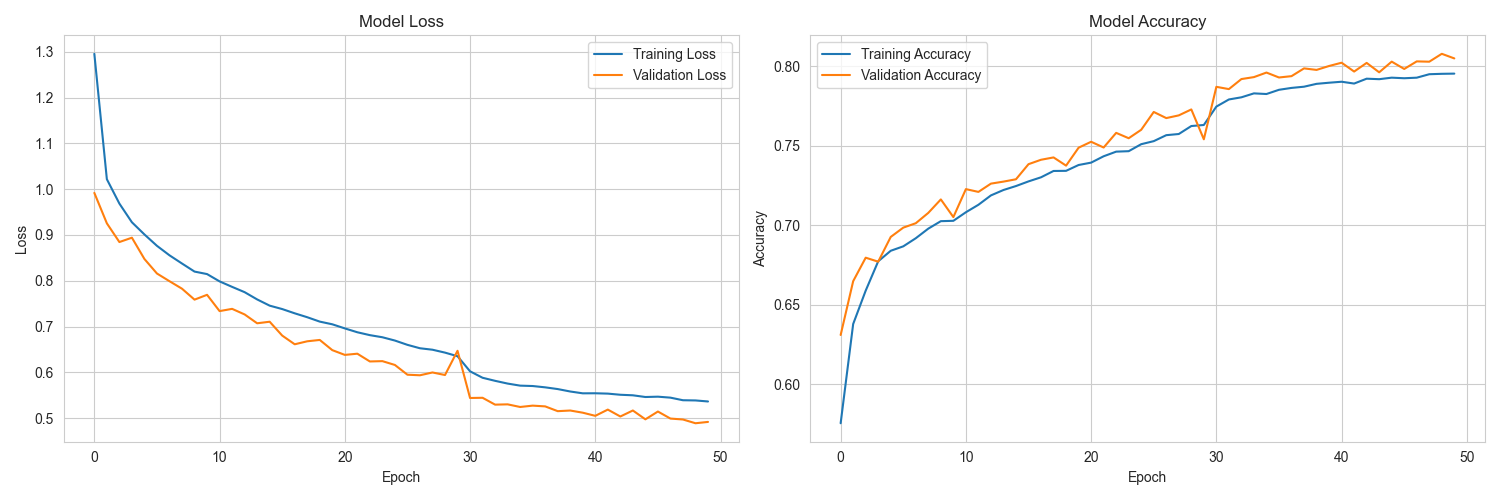
\includegraphics[width=0.8\textwidth]{data/models/ids_model_20250604_081352/training_history.png}
  \caption{Courbes d'apprentissage du modèle entraîné le 2025-06-04. On observe la loss et l'accuracy sur l'entraînement et la validation.}
\end{figure}

\begin{figure}[h!]
  \centering
  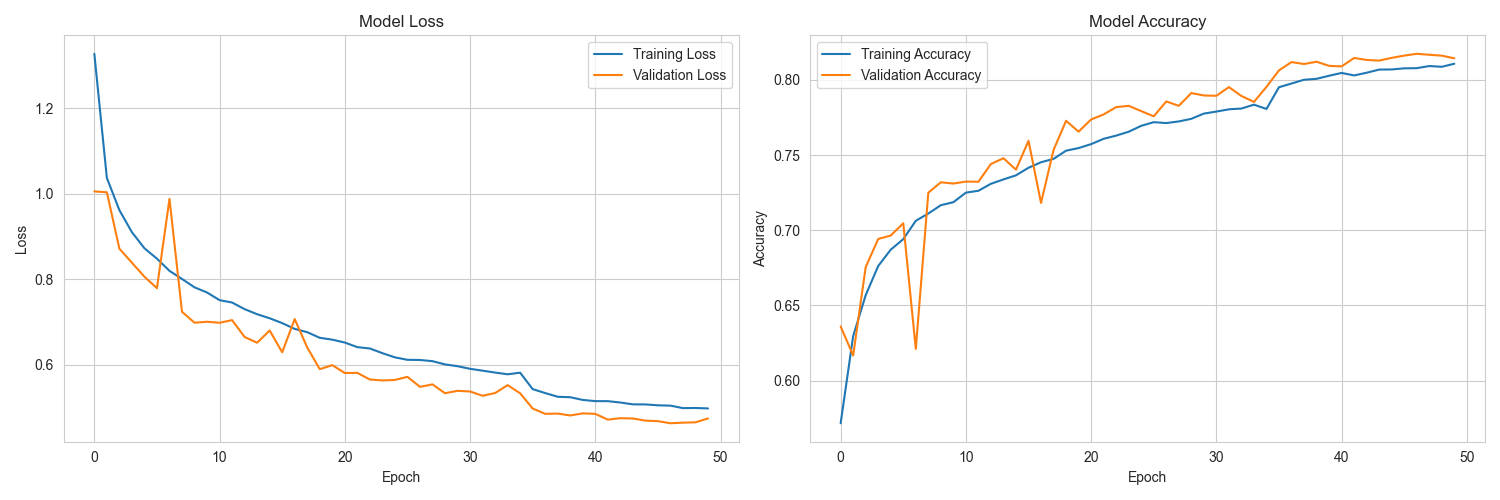
\includegraphics[width=0.8\textwidth]{data/models/ids_model_20250717_140013/training_history.png}
  \caption{Courbes d'apprentissage du modèle entraîné le 2025-07-17. Comparer la stabilité et la performance des courbes de validation pour choisir le meilleur modèle.}
\end{figure}

%%%%%%%%%%%%%%%%%%%%%%%%%%%%%%%%%%%%%%%%%%%%%%%%%%%%%%%%%%%%
\section{Questions complémentaires sur le backend IA}

\subsection{Comment le modèle est-il sauvegardé et rechargé ?}
Le modèle entraîné est sauvegardé dans un dossier dédié (par exemple \texttt{data/models/ids\_model\_20250604\_081352/}) sous forme de fichiers TensorFlow/Keras. Le code utilise la méthode \texttt{model.save()} pour la sauvegarde et \texttt{tf.keras.models.load\_model()} pour le rechargement. Les objets de normalisation (scaler) et d'encodage des labels sont également sauvegardés pour garantir la cohérence lors des prédictions futures.

\begin{lstlisting}[language=Python]
self.model.save(model_path)
# ...
model = tf.keras.models.load_model(model_path)
\end{lstlisting}

\subsection{Comment faire une prédiction sur une nouvelle donnée ?}
Pour prédire si une connexion réseau est une attaque, il faut :
\begin{enumerate}
  \item Prétraiter la donnée (extraction et normalisation des features)
  \item Appliquer le modèle pour obtenir la prédiction
  \item Interpréter la sortie (classe prédite)
\end{enumerate}
Cela se fait via la méthode \texttt{predict()} du modèle, après avoir transformé la donnée d'entrée au bon format.

\begin{lstlisting}[language=Python]
predictions = model.predict(X)
predicted_class = np.argmax(predictions[0])
\end{lstlisting}

\subsection{Comment sont gérés les logs de tests ?}
Après chaque prédiction ou test, un log est enregistré dans un fichier JSON (\texttt{data/test\_logs.json}). Chaque log contient l'entrée, la prédiction, la classe réelle (si connue), la confiance, et le statut (succès/échec). Cela permet de suivre l'historique des performances du modèle et de diagnostiquer d'éventuelles erreurs.

\begin{lstlisting}[language=Python]
log_entry = {
    'timestamp': datetime.now().isoformat(),
    'testType': 'Validation',
    'input': str(X_val[i].flatten().tolist()),
    'prediction': int(y_pred_labels[i]),
    'confidence': float(y_pred[i].max()),
    'true_class': int(y_val_labels[i]),
    'status': 'success' if y_pred_labels[i] == y_val_labels[i] else 'fail'
}
\end{lstlisting}

\subsection{Quelles sont les limites du modèle actuel ?}
Le modèle dépend fortement de la qualité et de la diversité des données d'entraînement. Il peut avoir du mal à détecter des attaques très différentes de celles vues pendant l'entraînement (généralisation limitée). De plus, il n'y a pas de gestion automatique de la mise à jour du modèle en production, ni de détection d'attaques inconnues (zero-day).

\subsection{Comment ajouter un nouveau type d'attaque ?}
Pour ajouter un nouveau type d'attaque, il faut :
\begin{enumerate}
  \item Ajouter la nouvelle classe dans la variable \texttt{ATTACK\_TYPES} du code.
  \item S'assurer que les données d'entraînement contiennent des exemples de cette attaque.
  \item Réentraîner le modèle pour qu'il apprenne à la reconnaître.
\end{enumerate}

\subsection{Comment le backend gère-t-il la scalabilité ou la mise à jour du modèle ?}
Actuellement, le backend charge le modèle en mémoire et l'utilise pour toutes les prédictions. Pour mettre à jour le modèle, il faut réentraîner et sauvegarder un nouveau modèle, puis redémarrer le service pour qu'il charge la nouvelle version. Il n'y a pas encore de mécanisme automatique de mise à jour ou de gestion de plusieurs versions en parallèle.

\subsection{Comment sont gérées les erreurs ou les cas inattendus ?}
Le code prévoit des blocs \texttt{try/except} pour capturer les erreurs lors des prédictions ou du chargement du modèle. En cas d'erreur, un message explicite est retourné et, dans certains cas, une prédiction simulée est renvoyée pour éviter de bloquer le système.

\begin{lstlisting}[language=Python]
try:
    # ... prediction
except Exception as e:
    print(f"Erreur lors de la prediction : {str(e)}")
    # ... prediction simulee
\end{lstlisting}

%%%%%%%%%%%%%%%%%%%%%%%%%%%%%%%%%%%%%%%%%%%%%%%%%%%%%%%%%%%%
\section{Frontend : Interface utilisateur Next.js}

\subsection{Présentation générale}
Le frontend du projet est développé avec Next.js, un framework moderne basé sur React. Il permet de créer une interface utilisateur réactive, ergonomique et facilement maintenable. Le code source se trouve dans le dossier \texttt{frontend-next/}.

\subsection{Organisation et architecture}
Le projet est organisé en pages (\texttt{src/app/}) et en composants réutilisables (\texttt{src/components/}). Chaque page correspond à une vue principale de l'application (dashboard, alertes, règles, paramètres, etc.).

\subsection{Rôle de Next.js et des fichiers principaux}
Next.js gère le routage, le rendu côté client, et l'organisation des pages. Les fichiers importants sont :
\begin{itemize}
  \item \texttt{src/app/layout.tsx} : structure globale de l'application (sidebar, layout)
  \item \texttt{src/app/page.tsx} : page d'accueil (redirection)
  \item \texttt{src/app/dashboard/page.tsx} : tableau de bord principal
  \item \texttt{src/app/alerts/page.tsx} : affichage des alertes
  \item \texttt{src/app/settings/page.tsx} : configuration des paramètres
  \item \texttt{src/components/} : composants réutilisables (tableaux, graphiques, formulaires, etc.)
\end{itemize}

\subsection{Communication avec le backend}
Le frontend communique avec le backend Flask via des appels API HTTP (principalement avec \texttt{fetch}). Les endpoints utilisés sont par exemple :
\begin{itemize}
  \item \texttt{/api/stats/traffic} : données réseau en temps réel
  \item \texttt{/api/stats/alerts} : liste des alertes
  \item \texttt{/api/settings} : lecture et modification des paramètres
  \item \texttt{/api/rules} : gestion des règles IDS
\end{itemize}

\textbf{Exemple d'appel API dans un composant React :}
\begin{lstlisting}[language=JavaScript]
useEffect(() => {
    fetch('http://localhost:5000/api/stats/alerts')
        .then(res => res.json())
        .then(setAlerts);
}, []);
\end{lstlisting}

\subsection{Gestion de l'état et des effets}
L'état de l'application est géré avec les hooks React \texttt{useState} et \texttt{useEffect}. Par exemple, pour stocker et mettre à jour la liste des alertes :
\begin{lstlisting}[language=JavaScript]
const [alerts, setAlerts] = useState<Alert[]>([]);
useEffect(() => {
    fetch('http://localhost:5000/api/stats/alerts')
        .then(res => res.json())
        .then(setAlerts);
}, []);
\end{lstlisting}

Des hooks personnalisés (ex : \texttt{useNetworkData}) sont utilisés pour centraliser la logique de récupération des données réseau.

\subsection{Composants principaux}
\begin{itemize}
  \item \textbf{Dashboard} : vue d'ensemble des métriques, historique, logs de tests
  \item \textbf{AlertsTable} : affichage des alertes récentes
  \item \textbf{SettingsPage} : gestion des paramètres (seuils, modules actifs)
  \item \textbf{RulesPage} : gestion dynamique des règles IDS
  \item \textbf{ModelStats, NetworkTraffic, SystemStats} : visualisation des statistiques et graphiques
\end{itemize}

\subsection{Gestion des erreurs et du chargement}
Chaque appel API gère les états de chargement et d'erreur pour informer l'utilisateur :
\begin{lstlisting}[language=JavaScript]
const [loading, setLoading] = useState(true);
const [error, setError] = useState<string | null>(null);

useEffect(() => {
    fetch('http://localhost:5000/api/stats/alerts')
        .then(res => res.json())
        .then(data => {
            setAlerts(data);
            setLoading(false);
        })
        .catch(() => {
            setError('Erreur lors du chargement des alertes.');
            setLoading(false);
        });
}, []);
\end{lstlisting}

\subsection{Bibliothèques externes utilisées}
Le frontend utilise plusieurs bibliothèques pour améliorer l'expérience utilisateur :
\begin{itemize}
  \item \texttt{react} et \texttt{next} : base du framework
  \item \texttt{tailwindcss} : styles et design moderne
  \item \texttt{recharts} : graphiques interactifs
  \item \texttt{react-hook-form} : gestion des formulaires
  \item \texttt{sonner} : notifications
  \item \texttt{lucide-react} : icônes
\end{itemize}

\subsection{Résumé visuel de l'architecture frontend}
\begin{itemize}
  \item Sidebar (navigation)
  \item Pages principales (Dashboard, Alertes, Règles, Paramètres)
  \item Composants réutilisables (tableaux, graphiques, formulaires)
\end{itemize}

L'architecture modulaire permet de faire évoluer facilement l'interface et d'ajouter de nouvelles fonctionnalités.

% (La suite : Frontend, API, etc. à compléter...)

\end{document} 